\documentclass[letterpaper,11pt, spanish]{article}

%acentos de la forma ´ en vez de \'a
\usepackage[utf8]{inputenc}
\usepackage{babel}
\makeatletter

\usepackage[letterpaper]{geometry}

\usepackage{hyperref}
\usepackage{graphicx}
\usepackage{setspace}
\usepackage{color}
\usepackage{hyperref}
\usepackage{amssymb}
\usepackage{url}
%\usepackage{pdfpages}
\usepackage{fancyhdr}
\usepackage{hyperref}
\usepackage{amsmath}
\usepackage{amsthm}
\usepackage{booktabs}
\usepackage{subfig}
\usepackage{tikz}
\usetikzlibrary{arrows,automata}
\usepackage{listings} %Codigo
\lstset{language=C, tabsize=4,framexleftmargin=5mm,breaklines=true}
\newenvironment{enumerate2}{
\begin{enumerate}
	\setlength{\itemsep}{0pt}
	\setlength{\parskip}{0pt}}{
\end{enumerate}
}

\begin{document}
\onehalfspace{}

%\begin{sf}

% --------------- ---------PORTADA --------------------------------------------
\newpage
\pagestyle{fancy}
\fancyhf{}
%-------------------- CABECERA ---------------------
\fancyhead[L]{Universidad de Chile \\ Facultad de Cs. Físicas y Matemáticas \\ Departamento de Ciencias de la Computación \\ CC5113 - 1}
\fancyhead[R]{
\includegraphics[scale=0.3]{LogoUIngenieria.png}}
%------------------ TÍTULO -----------------------
\vspace*{6cm}
\begin{center}
\Huge  {Aprendizaje Automático Bayesiano}\\
\vspace{1cm}
\huge {Definición de Proyecto} \\
\end{center}
%----------------- NOMBRES ------------------------
\vfill
\begin{flushright}
\begin{tabular}{ll}
& Autores: Vicente Oyanedel \\
& 			Francisco Clavero \\
& Profesor: Pablo Guerrero \\
& \today \\
& Santiago, Chile.
\end{tabular}
\end{flushright}

% ·············· ENCABEZADO - PIE DE PAGINA ············
\newpage
\pagestyle{fancy}
\fancyhf{}

%Encabezado
%\fancyhead[L]{\rightmark}
\fancyhead[L]{\small \rm \textit{Sección \rightmark}} %Izquierda


\fancyfoot[L]{\small \rm \textit{CC5113 - Vicente Oyanedel, Francisco Clavero}} %Izquierda
\fancyfoot[R]{\small \rm \textit{\thepage}} %Derecha
%\fancyfoot[C]{\thepage} %Centro

\renewcommand{\sectionmark}[1]{\markright{\thesection.\ #1}}
\renewcommand{\headrulewidth}{0.5pt}
\renewcommand{\footrulewidth}{0.5pt}

% =============== INDICE ===============

\tableofcontents

% =============== BLOQUE DECODIFICADOR ===============
\newpage
\section{Descripción General del Proyecto}

\href{las.leagueoflegends.com}{League of Legends} es un videojuego del estilo MOBA (Multiplayer Online Battle Arena),
donde dos equipos de 5 jugadores se enfrentan en una lucha por destruir el nexo
(base) enemigo. \\

\begin{figure}[h]
	\begin{center}
		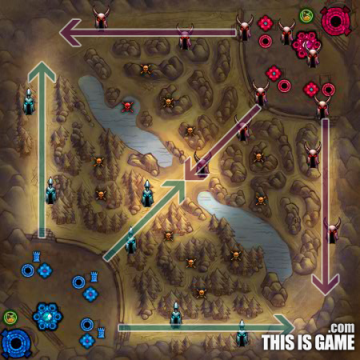
\includegraphics[scale=0.75]{map.png}
	\end{center}
	\caption{Mapa con los objetivos del juego.}
\end{figure}

Durante una partida, cada jugador puede controlar uno de aproximadamente 150 campeones
distintos. Cada uno tiene distintas habilidades y atributos, que determinan
su forma de uso, dificultad y proposito dentro del juego. Esto provoca que
los campeones sean muy distintos entre si, y que cada jugador tenga una afinidad
distinta por cada campeón, sea por gusto o por su rendimiento con ellos. La simplicidad
de los objetivos y a variedad de los campeones hace a League of Legends un juego
muy dinámico, a lo cual debe su fama. \\

Cada jugador tiene una cuenta de usuario con la cual se autentifica para jugar, y
almacena estadistidísticas de cada partida jugada. Esto incluye datos como
la cantidad de partidas jugadas, ganadas, o perdidas, la cantidad de contrincantes vencidos,
los campeones que ha usado, entre otros, con las cuales se puede caracterizar a
los usuarios. \\

El proyecto consiste en crear un sistema que recomiende campeones a un usuario de
League of Legends con los cuales pueda tener un buen rendimiento en el juego,
basado en las características de dicho usuario. \\

La recomendación se realiza en base a los campeones que utilizan usuarios con
características similares a las del usuario que ingresa al sistema. Para lograr
identificar los distintos grupos de usuarios similares, se utilizarán técnicas
de clustering. \\

\section{Alcances del Proyecto}

En primer lugar, los datos se obtienen mediante la \href{https://developer.riotgames.com/}{API oficial}
del juego, la cual provee un servicio de requests en formato json. Esta permite
acceder directamente a los datos de los $2000$ mejores usuarios del mundo (los $200$
mejores de $10$ regiones distintas). Si bien esto puede limitar la aplicabilidad
inicial del modelo, la API también provee métodos para acceder a los datos de los
demás usuarios mediante su id de usuario. Estos datos pueden ser incorporados
en etapas posteriores. \\

Usando la información da cada partida, es posible generar una función de rendimiento
de un usuario con un campeón en específico a partir de las distintas métricas
disponibles. De este modo, al identificar al usuario que ingresa al sistema
con uno de los clusters generados con los datos de entrenamientos, se le recomiendan
los campeones con mejor rendimiento promedio en el cluster. \\

\newpage
\section{Rol Específico de cada Integrante}

Se utilizará el software de control de versiones y coordinación GitHub, lo cual
permite que los integrantes puedan trabajar paralelamente en el proyecto, sin
la necesidad de especificar roles claros. La asignación de tareas específicas
quedará regitrada mediante la asignación de $issues$ en el
\href{https://github.com/fcoclavero/machinelol}{repositorio} de GitHub. \\

\section{Metodología}

Toda la programación será hecha en el lenguaje Python por diversas razones. en
primer lugar, las librerías $json$ y $requests$ facilitan la obtención de los
datos de la API, y su posterior manejo como base de dato basada en documentos
(en formato json). En segundo lugar, para realizar el clustering se utilizarán
los métodos de la librería de python $sklearn$, y la librería $numpy$ para
manejar los datos. \\

Como se mencionaba anteriormente, para organización y control de versión, se
utilizará GitHub.

% ============= FIN DE DOCUMENTO ==============
\end{document}

% % ················ IMAGEN ·················
% \begin{figure}[ht!]
% \centering
% \fbox{\includegraphics[scale=0.6]{img/flujo.png}}
% \caption{Flujo de caja anual}\label{flujo}
% \end{figure}
% %··········································

% % ················ IMAGEN DOBLE ·················
% \begin{figure}[ht!] \centering
% \subfloat[Esquemático]{\includegraphics[scale=0.44]{img/seguidor.png}}
% \subfloat[Simulación]{\includegraphics[scale=0.45]{img/seguidor1.png}}
% \caption{Simulación como seguidor de voltaje}\label{seguidor}
% \end{figure}
% %··········································

%% ............... INSERTAR IMAGEN ......................
% \begin{center}
%	\includegraphics[scale=0.75]{Imagenes/circuito.jpg}
% \end{center}

% ............... INSERTAR CODIGO ......................
% \begin{center}
% 	\lstinputlisting{Circuitos/log.txt}
% \end{center}
